\newpage
\section{Sistemas de Coordenadas}

\subsection{Cilíndricas}

\begin{table}[H]
    \centering
    \begin{tabular}{|c|c|}
        \hline
        $x = {\rho}cos(\phi)$ & $\rho = \sqrt{x^2 + y^2}$ \\
        \hline
        $y = {\rho}sin(\phi)$ & $\phi = atan(\frac{y}{x})$ \\
        \hline
    \end{tabular}
\end{table}

\begin{figure}[H]
    \centering
    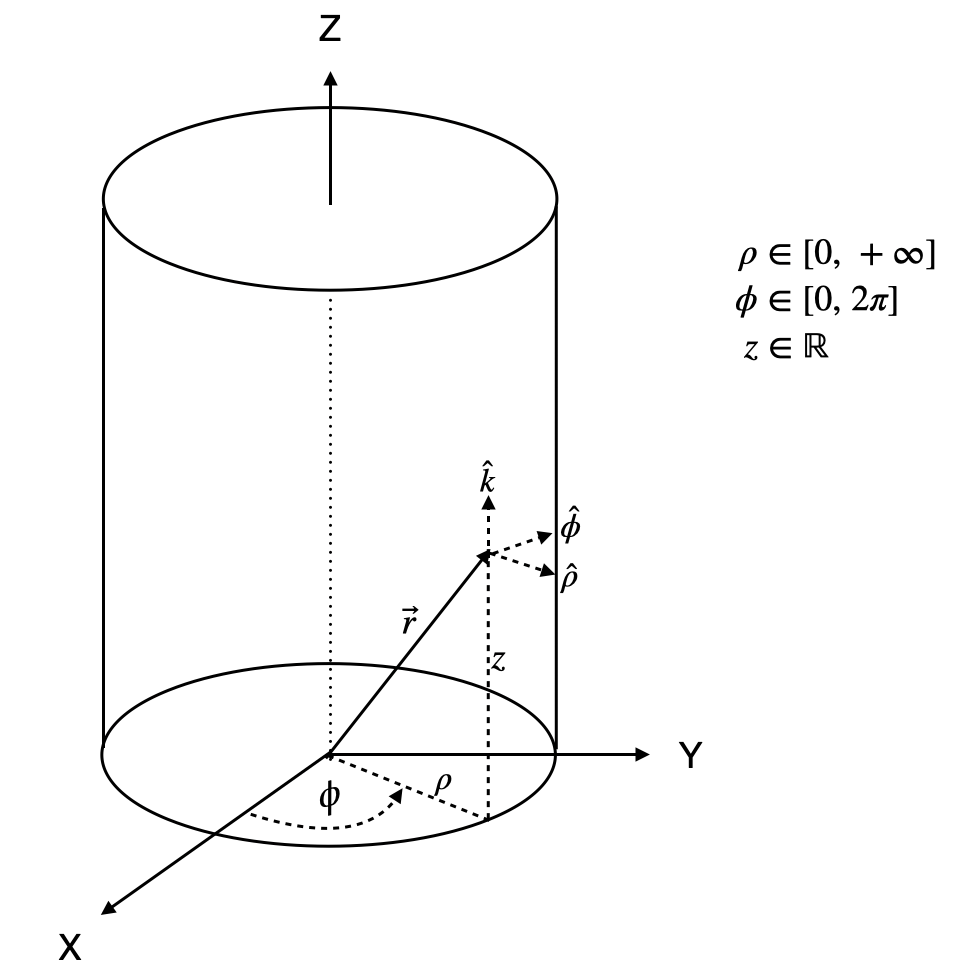
\includegraphics[width=0.6\textwidth]{Cosas Matemáticas/coords_cilind_DFI.png}
    \caption{Coordenadas cilíndricas en el plano cartesiano}
    \label{fig:C.cilindricas}
\end{figure}

Vectores unitarios:

\begin{itemize}
    \item $\hat{z}$: Es el mismo que en cartesianas
    \item $\hat{\rho}$: Apunta en dirección del radio
        \[\hat{\rho} = cos(\phi)\hat{x} + sin(\phi)\hat{y}\]
    \item $\hat{\phi}$: Apunta en la dirección en que el ángulo $\phi$, formado por el radio y el eje x, se expande. %En DIM lo denotan como $\hat{\theta}$
        \[\hat{\phi} = -sin(\phi)\hat{x} + cos(\phi)\hat{y}\]
\end{itemize}

\medbreak

Derivadas temporales de los vectores unitarios:

\begin{itemize}
    \item $\dot{\hat{\rho}} = \dot{\phi}\hat{\phi}$
    \item $\dot{\hat{\phi}} = -\dot{\phi}\hat{\rho}$
\end{itemize}

\medbreak

Posición, velocidad y aceleración:

\begin{itemize}
    \item $\vec{r} = \rho\hat{\rho} + z\hat{z}$
    \item $\vec{v} = \dot{\rho}\hat{\rho} + \rho\dot{\phi}\hat{\phi} + \dot{z}\hat{z}$
    \item $\vec{a} = (\ddot{\rho}-\rho\dot{\phi}^2)\hat{\rho} + (\rho\ddot{\phi}+2\dot{\rho}\dot{\phi})\hat{\phi} + \ddot{z}\hat{z}$
\end{itemize}

\medbreak

Gradiente:

\[\nabla F = \frac{\partial F}{\partial \rho}\hat{\rho} + \frac{1}{\rho}\frac{\partial F}{\partial \phi}\hat{\phi} + \frac{\partial F}{\partial z}\hat{z}\]

Divergencia:

\[\nabla \cdot \vec{F} = \frac{1}{\rho}\left(\frac{\partial(F_{\rho}\rho)}{\partial\rho}+\frac{\partial F_{\phi}}{\partial\phi}+\frac{\partial(F_{z}\rho)}{\partial z}\right)\]

Rotor:
% Elimine un rho que acompañaba a dF_phi/dphi
\[\nabla\times\vec{F} = \frac{1}{\rho}\left(\frac{\partial F_{z}}{\partial \phi}-\rho\frac{\partial F_{\phi}}{\partial z}\right)\hat{\rho} + \left(\frac{\partial F_{\rho}}{\partial z}-\frac{\partial F_{z}}{\partial \rho}\right)\hat{\phi} + \frac{1}{\rho}\left(\frac{\partial(F_{\phi}\rho)}{\partial \rho}-\frac{\partial F_{\rho}}{\partial \phi}\right)\hat{z}\]

\medbreak

Diferenciales:

\begin{itemize}
    \item Linea:
    \[d\vec{r} = d\rho\hat{\rho} + \rho d\phi\hat{\phi}+dz\hat{z}\]
    \item Superficie:
    \[d\vec{S} = \rho d\phi dz\hat{\rho}+d\rho dz\hat{\phi}+\rho d\rho d\phi\hat{z}\]
    \item Volumen:
    \[dV = \rho d\rho d\phi dz\]
\end{itemize}

\newpage

\subsection{Esféricas}

\begin{table}[h]
    \centering
    \begin{tabular}{|c|c|}
        \hline
        $x = rsin(\theta)cos(\phi)$ & $r = \sqrt{x^2 + y^2 + z^2}$ \\
        \hline
        $y = rsin(\theta)sin(\phi)$ & $\phi = atan(\frac{y}{x})$ \\
        \hline
        $z = rcos(\theta)$ & $\theta = atan(\frac{\sqrt{x^2+ y^2}}{z})$ \\
        \hline
    \end{tabular}
\end{table}

\begin{figure}[H]
    \centering
    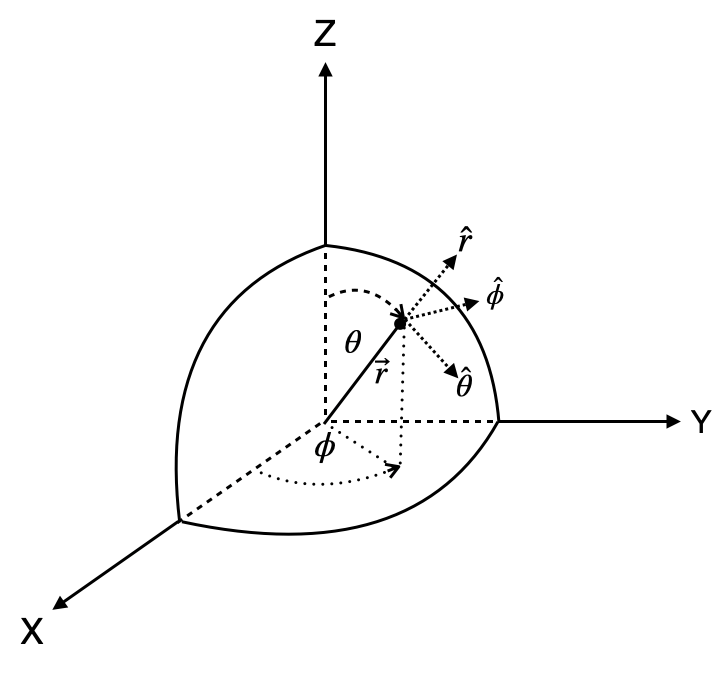
\includegraphics[width=0.7\textwidth]{Cosas Matemáticas/coords_esferc_DFI.png}
    \caption{Coordenadas esféricas en el plano cartesiano}
    \label{fig:C.esfericas}
\end{figure}

Vectores unitarios:

\begin{itemize}
    \item $\hat{r}$: Apunta en dirección del radio
        \[\hat{r} = sin(\theta)cos(\phi)\hat{x} + sin(\theta)sin(\phi)\hat{y} + cos(\theta)\hat{z}\]
    \item $\hat{\phi}$: Apunta en la dirección en que el ángulo $\phi$, formado por la proyección del radio en el plano xy y el eje x, se expande. %En DIM lo denotan como $\hat{\theta}$
        \[\hat{\phi} = -sin(\phi)\hat{x} + cos(\phi)\hat{y}\]
    \item $\hat{\theta}$: Apunta en la dirección en que se expande el ángulo $\theta$, formado por el radio y el eje z. %En DIM lo denotan como $\hat{\varphi}$
        \[\hat{\theta} = cos(\theta)cos(\phi)\hat{x} + cos(\theta)sin(\phi)\hat{y}-sin(\theta)\hat{z}\]
\end{itemize}

\medbreak

Derivadas temporales de los vectores unitarios:

\begin{itemize}
    \item $\dot{\hat{r}} = \dot{\phi}cos(\theta)\hat{\phi}+\dot{\theta}\hat{\theta}$
    \item $\dot{\hat{\phi}} = -\dot{\phi}(sin(\theta)\hat{r}+cos(\theta)\hat{\theta})$
    \item $\dot{\hat{\theta}} = -\dot{\theta}\hat{r}+\dot{\phi}cos(\theta)\hat{\phi}$
\end{itemize}

\medbreak

Posición, velocidad y aceleración:

\begin{itemize}
    \item $\vec{r} = r\hat{r}$
    \item $\vec{v} = \dot{r}\hat{r} + r(\dot{\phi}cos(\theta)\hat{\phi}+\dot{\theta}\hat{\theta})$
    \item $\vec{a} = (\ddot{r}-r\dot{\theta}^2-r\dot{\phi}^2sin^2(\theta))\hat{r} + (r\ddot{\theta}+2\dot{r}\dot{\theta}+r\dot{\phi}^2sin(\theta)cos(\theta))\hat{\theta} + \frac{d(r^2\dot{\phi}sin^2(\theta))}{dt}\frac{1}{rsin(\theta)}\hat{\phi}$
\end{itemize}

\medbreak

Gradiente:

\[\nabla F = \frac{\partial F}{\partial r}\hat{r} + \frac{1}{rsin(\theta)}\frac{\partial F}{\partial \phi}\hat{\phi} + \frac{1}{r}\frac{\partial F}{\partial \theta}\hat{\theta}\]

Divergencia:

\[\nabla \cdot \vec{F} = \frac{1}{r^2sin(\theta)}\left(\frac{\partial(F_{r}r^2sin(\theta))}{\partial r}+\frac{\partial (F_{\phi}r)}{\partial\phi}+\frac{\partial(F_{\theta}rsin(\theta))}{\partial \theta}\right)\]

Rotor:

\[\nabla\times\vec{F} = \frac{1}{r\sin\theta} \left( \frac{\partial}{\partial \theta} \left(F_\phi\sin\theta \right) - \frac{\partial F_\theta}{\partial \phi} \right) \hat{r} + \frac{1}{r} \left( \frac{1}{\sin\theta} \frac{\partial F_r}{\partial \phi} - \frac{\partial}{\partial r} \left( r F_\phi \right) \right) \hat{\theta} + \frac{1}{r} \left( \frac{\partial}{\partial r} \left( r F_{\theta} \right) - \frac{\partial F_r}{\partial \theta} \right) \hat{\phi}\]

Diferenciales:

\begin{itemize}
    \item Linea:
    \[d\vec{r} = dr\hat{r} + rsin(\theta) d\phi\hat{\phi}+rd\theta\hat{\theta}\]
    \item Superficie:
    \[d\vec{S} = r^2sin(\theta)d\phi d\theta\hat{r}+rdrd\theta\hat{\phi}+rsin(\theta)dr d\phi\hat{\theta}\]
    \item Volumen:
    \[dV = r^2sin(\theta)d\rho d\phi d\theta\]
\end{itemize}

\newpage